\chapter{Simulation, Reconstruction and Event Selections}
\label{chap:Selections}

\section{Simulation}
\label{sec:Selections_Simulation}

In order to generate a Monte Carlo prediction of the expected event rate at the far detector for both sets of samples, all the processes in the beamline, atmospheric flux, neutrino interaction and detector need to be modelled. The beamline simulation consists of three distinct parts; initial hadron interaction modelling, target station geometry and particle tracking and hadronic re-interactions. These are modelled by FLUKA \cite{fluka2011}, JNUBEAM \cite{geant3, PhysRevD.87.012001} and GCALOR \cite{gcalor}, respectively. FLUKA is not very adaptable but matches external cross-section measurements in the region of interest better than GCALOR (\quickmath{O(10)\text{GeV}}). Thus a small simulation is built to model the interactions in the target and the output is then passed to JNUBEAM and GCALOR for propagation. The hadronic interactions are tuned to data from the NA61/SHINE \cite{Abgrall_2011, Abgrall_2012, NA61_pions_rep} and HARP \cite{harp} experiments. The tuning is done by reweighting the FLUKA and GCALOR predictions to match the external data multiplicity and cross-section measurements, based on final state particle kinematics \cite{t2k_tn_flux}. The predicted flux for neutrino and antineutrino beam modes is illustrated in \autoref{fig:T2KSKExp_T2K_NuFluxPerMode}.

The atmospheric neutrino flux predictions are simulated by the HKKM model \cite{Honda_2007, Honda:2011}, where the primary cosmic ray flux is tuned to AMS \cite{Blau2002} and BESS \cite{Haino2004} external data assuming the US-standard atmosphere `76 \cite{USStandardAtm} density profile and includes geomagnetic field effects. Secondary interactions of pions and muons are handled by DPMJET-III \cite{Roesler2001} for energies above \quickmath{32\text{GeV}} and JAM \cite{Niita2006, Honda:2011} for energies below that value. These hadronic interactions are tuned to external data \cite{Sanuki_2002, Achard_2004} using the same methodology as the tuning of the beamline simulation. The energy and cosine zenith predictions of \quickmath{\nu_{e}, \bar{\nu}_{e}, \nu_{\mu}, \bar{\nu}_{\mu}} flux are given in \autoref{fig:NeutrinoOscillationPhysics_AtmosphericNeutrinoFlux} and \autoref{fig:NeutrinoOscillationPhysics_NuFluxZenithAngleDep}, respectively. The flux is approximately symmetrical and peaked around \quickmath{\cos(\theta_{Z}) = 0.0}. This is because horizontally-going pions and kaons can travel further than their vertically-going counterparts resulting in a larger probability of decay to neutrinos. The symmetry is broken in low-energy neutrinos due to geomagnetic effects, which modify the track of the primary cosmic rays.

The neutrino interactions in all three detectors are simulated with NEUT \cite{Hayato2021, neut}. This simulates quasi-elastic (QE), meson exchange (MEC), single meson production (PROD), coherent pion production (COH) and deep inelastic scattering (DIS) interactions. These interaction categories can be further broken down by whether they were propagated via a \quickmath{W^{\pm}} boson in Charged Current (CC) interactions or via a \quickmath{Z^{0}} boson in Neutral Current (NC) interactions. CC interactions have a charged lepton in the final state, which can be flavour-tagged in reconstruction to determine the flavour of the neutrino. In contrast, NC interactions have a neutrino in the final state so no flavour information can be determined from the observables in the detector. This is the reason why NC events are assumed to not oscillate within the analysis. Both CC and NC interactions are modelled for all the above interaction categories, other than MEC interactions which are only modelled for CC events. The SK detector is only sensitive to charged particles, so all charged current interactions are simulated whilst only neutral current processes which produce charged mesons (NCDIS, NCCOH and NCPROD) are modelled. NC MEC interactions can only produce charged particles through secondary re-interactions which is a low cross-section process.

\begin{figure}[h]
  \begin{subfigure}[t]{0.8\textwidth}
    \includegraphics[width=\textwidth, trim={0mm 0mm 0mm 0mm}, clip,page=1]{Figures/Selections/NEUTCrossSection.pdf}
  \end{subfigure}
  \caption{The NEUT prediction of the \quickmath{\nu_{\mu}}-H2O cross-section overlaid on the T2K \quickmath{\nu_{\mu}} flux. The charged current (black, solid) and neutral current (black, dashed) inclusive, charged current quasi-elastic (blue, solid), charged current 2p2h (blue, dashed), charged current single pion production (pink) and charged current multi--\quickmath{\pi} and DIS (Purple) cross-sections are illustrated. Taken from \cite{Hayato2021}}
  \label{fig:Selection_CrossSection}
\end{figure}

As illustrated in \autoref{fig:Selection_CrossSection}, QE interactions dominate the low-energy cross-section of neutrino interactions. The NEUT implementation adopts the Llewellyn Smith \cite{llewelyn-smith} model for neutrino-nucleus interactions, where the nuclear ground state of any bound nucleons (neutrino-oxygen interactions) is approximated by a spectral-function \cite{Benhar1989} model that simulates the effects of Fermi momentum and Pauli blocking. The cross-section of QE interactions are controlled by vector and axial-vector form factors parameterised by the BBBA05 \cite{bbba05} model and a dipole form factor with \quickmath{M_{A}^{QE} = 1.21\text{GeV}} fit to external data \cite{Aguilar_Arevalo_2010}, respectively. QE interactions only account for single-nucleon interactions whereas multi-nucleon interactions (or MEC) can contribute significantly to the overall cross-section. NEUT implements the Valencia \cite{nieves2} model to simulate MEC events, where two nucleons and two holes in the nuclear target are produced (Often called 2p2h interactions due to this effect).

For neutrinos of energy \quickmath{O(1)\text{GeV}}, PROD interactions become dominant. These predominantly produce charged and neutral pions although \quickmath{\gamma}, kaon and \quickmath{\eta} production is also considered. To simulate these interactions, the Rein-Sehgal \cite{Rein_Sehgal} model is implemented within NEUT. It simulates the excitation of a nucleon from a neutrino interaction, production of an intermediate baryon, and the consequential decay to a single meson or \quickmath{\gamma}. Pions can also be produced through COH interactions, which occur when the incoming neutrino interacts with the entire oxygen nuclei target leaving a single pion outside of the nucleus. NEUT utilises the Berger-Sehgal \cite{Berger_Sehgal_coh} model to simulate these interactions.

DIS and multi-\quickmath{\pi} producing interactions become the most dominant for energies \quickmath{>O(5)\text{GeV}}. PYTHIA \cite{Sjstrand1994} is used to simulate any interaction with invariant mass, \quickmath{W > 2\text{GeV/c}^{2}}, which produces at least one meson. For any interaction which produces at least two mesons but has \quickmath{W < 2\text{GeV/c}^{2}}, the Bronner model is invoked \cite{Bronner2016}. Both of these models use Parton distribution functions based on the Bodek-Yang model \cite{Gl_ck_1998,10.48550/arxiv.1011.6592,10.48550/arxiv.1012.0261}. 

\begin{figure}[h]
  \begin{subfigure}[t]{0.8\textwidth}
    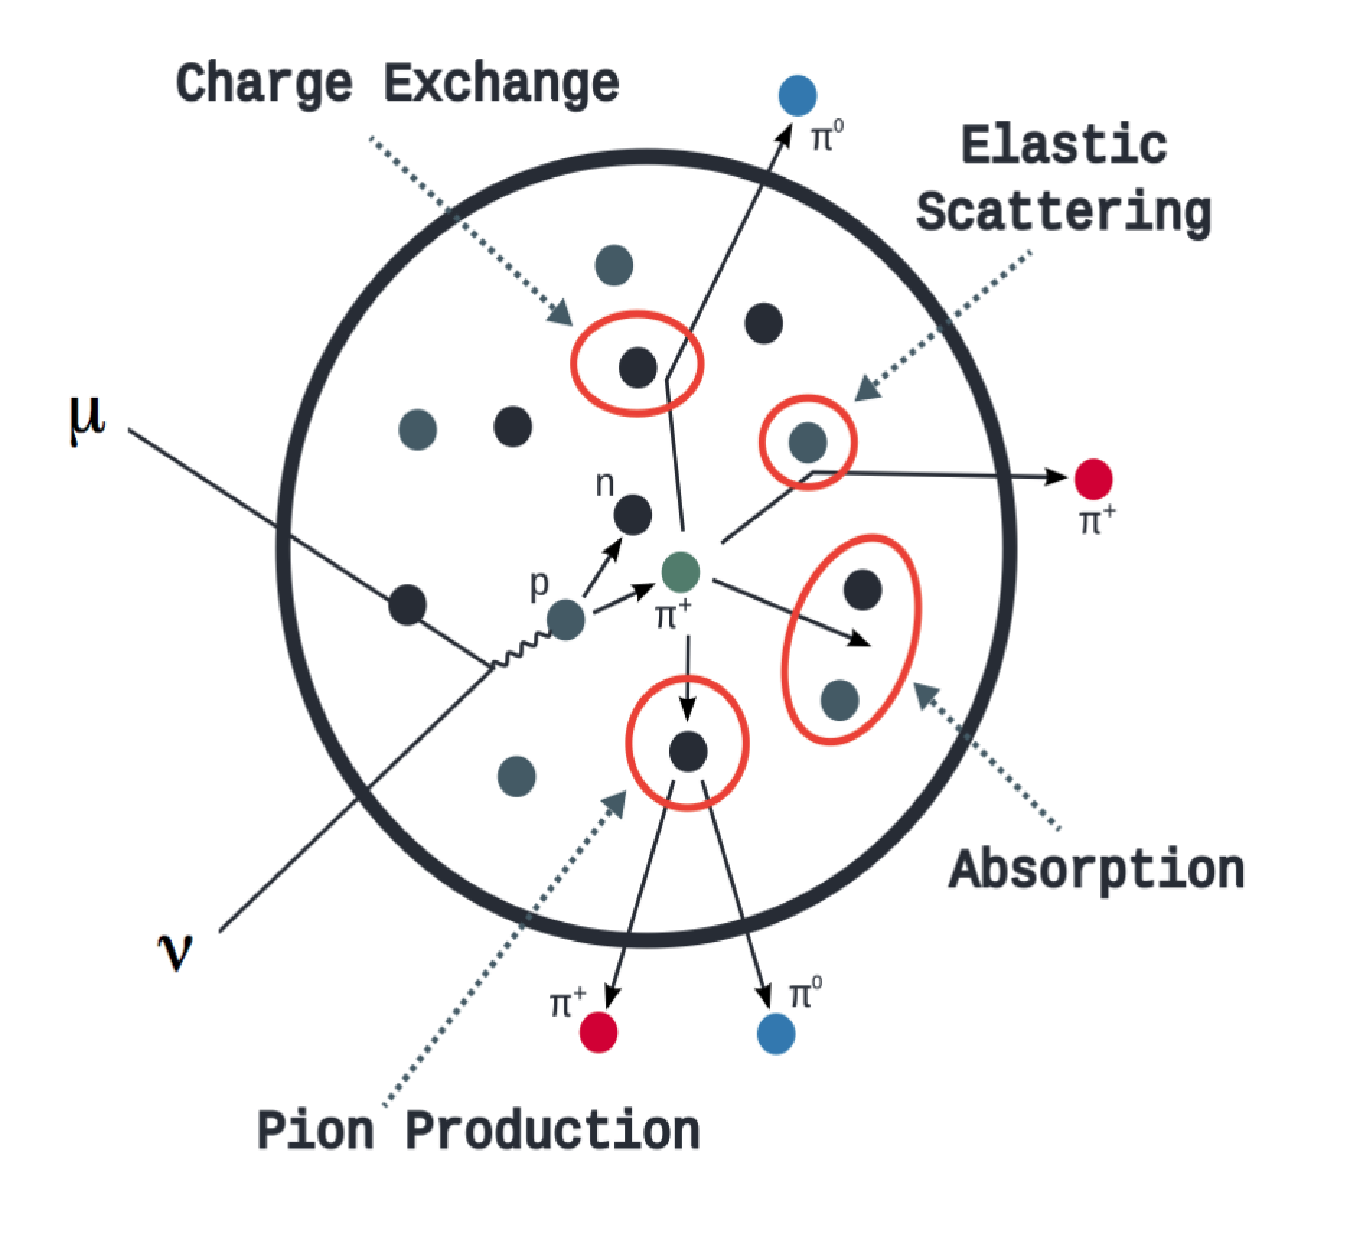
\includegraphics[width=\textwidth, trim={0mm 0mm 0mm 0mm}, clip,page=1]{Figures/Selections/FSIDiagram.pdf}
  \end{subfigure}
  \caption{Illustration of the various processes which a pion can undergo before exiting the nucleus. Taken from \cite{10.48550/arxiv.1602.05299}}
  \label{fig:Selection_FSIDiagram}
\end{figure}

Any pion which is produced within the nucleus can re-interact through final state interactions before it exits, as illustrated by the scattering, absorption, production and exchange interactions in \autoref{fig:Selection_FSIDiagram}. These re-interactions alter the observable particles within the detector. For instance, if the charged pion from a CC PROD interaction is absorbed, the observables would mimic a CC QE interaction. To simulate these effects, NEUT uses a semi-classical intranuclear cascade model \cite{Hayato2021}. This cascade functions by stepping the pion through the nucleus in fixed-length steps equivalent to \quickmath{dx = R_{N}/100}, where \quickmath{R_{N}} is the radius of the nucleus. At each step, the Monte Carlo allows the pion to interact through scattering, charged exchange, absorption or production with an interaction-dependent probability calculated from a fit to external data \cite{PhysRevD.99.052007}. This cascade continues until the pion is absorbed or exits the nucleus.

Once the outgoing particle kinematics have been determined from NEUT, they are passed into the detector simulation. The near detectors ND280 and INGRID are simulated using a \texttt{GEANT4} package \cite{t2k_det,geant4} to simulate the detector geometry and particle tracking. The response of the detectors is simulated using the elecSim package. The far detector simulation is based upon the original Kamiokande experiment software which uses the \texttt{GEANT3}-based SKDETSIM \cite{Brun:1987ma,t2k_det} package. This controls the interactions of particles in the water as well as Cherenkov light production. The water quality and PMT calibration measurements detailed in \autoref{subsec:T2KSKExp_SKCalibration} are also used within this simulation to make accurate predictions of the detector response.

\section{Event Reconstruction}
\label{sec:Simulation_Reconstruction}

\section{Event Selection}
\label{sec:Selections_Selection}
